%\setcounter{section}{0}
%\setcounter{subsection}{0}
%\setcounter{subsubsection}{0}
%\setcounter{equation}{0}
%\pagenumbering{arabic} 
%\setcounter{page}{0}    %%%%%KKD used \setcounter{page}{0}  
%\oddsidemargin 0.9 cm 
%\evensidemargin -.4 cm
%\setlength{\textwidth}{152.4 mm}
\newcommand{\pt}{ p_{T}}


\chapter{Advanced Pileup Mitigation Techniques  \label{ Advanced Pileup Mitigation Techniques}}



The performance of jets is extremely important to the success of most physics analyses. One of the outstanding challenges of the LHC run is the increase of instantaneous luminosity, which results in a large number of additional proton-proton collisions in each event(pileup). In such high pileup environment, the accurate reconstruction of jet properties and shapes becomes more and more demanding. The most common observables for jets are their $\rm p_{T}$, $\eta$, and $\phi$. Pileup changes the structure of jets by adding a lot of unwanted soft and wide-angle particles to them. In those cases the internal substructure of the jet contains information about the pileup contamination. In this part of the study, we have exploited the internal structure of the jet to get rid of the unwanted contaminations coming from pileup. The commonly used term `jet grooming' has become increasingly popular in recent times. Grooming has been introduced for the first time in Ref.~\cite{Grooming} and is intended to remove soft and wide-angle radiations from the jet. It is typically used to reduce the overall jet mass of quark- and gluon-initiated jets while retaining the larger jet mass for jets originating from decays of heavy particles
such as the top quark and W/Z/H bosons. In presence of pileup, grooming can be used to reduce the dependence of jet mass on pileup.  
It should be noted that jet grooming, in general, alters the soft structure of the jet while other jet structure observables may rely on this soft structure.  

In this section, we explore the effect of grooming as a pileup mitigation method on large-radius jets (R=0.8,1.2) summarizing our work from Ref.~\cite{JMEPAS}. We consider the following grooming methods: pruning~\cite{Ellis:2009me}, trimming~\cite{Krohn:2009th}, modified mass drop tagger~\cite{Dasgupta:2013ihk}, and soft drop~\cite{Larkoski:2014wba}.

The pruning algorithm reclusters the constituents of the jet through the Cambridge-Aachen (CA) algorithm~\cite{Dokshitzer:1997in}, using the same distance parameter as of the jet. At each step in the clustering algorithm, the softer of the two particles $i$ and $j$ to be merged is removed when the following conditions are met:

\begin{align}
z_{ij} & = \frac{ {\rm min}(\rm p_{T_{\it i}},  p_{T_{\it j}})} {\rm p_{T_{\it i}} + p_{T_{\it j}}} < z_{\rm cut} 
\label{eq:Rij1}
\end{align}

\begin{align}
\Delta R_{ij} & = \frac{2 \times r_{\rm cut} \times m_J}{\rm p_{T}} > D_{\rm cut}
\label{eq:Rij2}
\end{align}

where $m_J$ and $\rm p_{T}$ are the mass and transverse momentum of the originally-clustered jet, and $z_{\rm cut}$ and $r_{\rm cut}$ are parameters of the algorithm. A pictorial of pruning algorithm is shown in Fig.~\ref{fig:pruning_picture}. A point to be noted is that in our case the reclustering is done using CA, even though in the picture two options of reclustering are mentioned.

\begin{figure}[h]
\centering
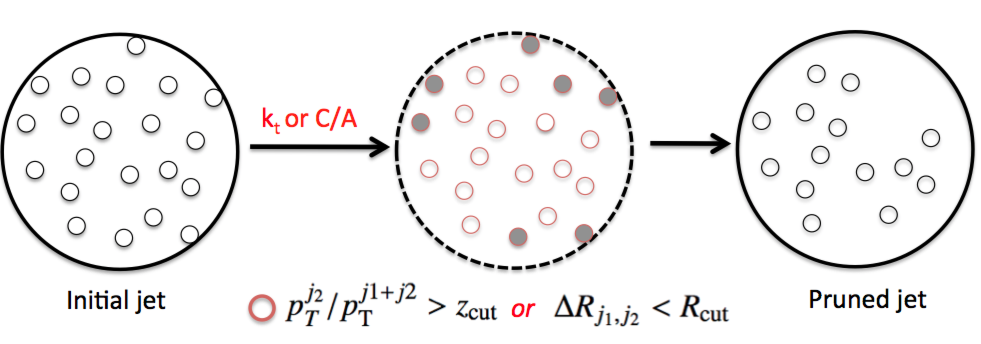
\includegraphics[width=0.7\textwidth]{/home/bibhu/Desktop/PhDThesis/PhDThesis/chapter8/pruning.png}
\caption{Pictorial representation of the pruning algorithm. The image is taken from Ref.~\cite{PruningPic}.}
\label{fig:pruning_picture}
\end{figure}


Trimming ignores particles within a jet that fall below a dynamic threshold in $\rm p_{T}$. 
It reclusters the constituents of the jet using the $k_{t}$ algorithm ~\cite{ktalgo} with a radius $R_{\rm sub}$, accepting only the subjets that have $\rm p_{T_{sub}} > f_{\rm cut} \lambda_{\rm hard}$, where $\rm f_{\rm cut}$ is a dimensionless cutoff parameter, and $\lambda_{\rm hard}$ is some hard QCD scale chosen to equal the $\rm p_{T}$ of the original jet. 






Soft-drop and modified mass drop tagger decluster the jet recursively removing soft and wide-angle radiation from the jet.
The jet is reclustered using the CA algorithm.  Then the jet is declustered and at each step, subjets $j_1$ and $j_2$ are defined to test  the following condition:

$\frac{{\rm min}(\rm p_{T_{j1}},\rm p_{T_{j2}})}{\rm p_{T_{j1}}+p_{T_{j2}}} > z_{\rm cut} \times \left( \frac{\Delta R_{12}}{R_0} \right)^{\beta}$

%\begin{align}
%\frac{{\rm min}(\pt_{j1},\pt_{j2})}{\pt_{j1}+\pt_{j2}} > z_{\rm cut} \times \left( \frac{\Delta R_{12}}{R_0} \right)^{\beta}
%\end{align}


where the algorithm parameters are $z_{\rm cut}$ and $\beta$.
If the condition is met, the declustering continues, otherwise only the leading $\rm p_{T}$ subjet is kept.
In the case when $\beta=0$, soft drop can be considered a generalization of the modified mass drop tagger.  

The (groomed) masses are corrected for pileup using a four-vector safe subtraction~\cite{Cacciari:2014jta}.
In the cases of soft drop, modified mass drop tagger, and trimming, the four-vector subtraction corrects the jet $\rm p_{T}$ and mass at each step in the algorithm.
For pruning, the correction is applied to the final product using the pruned jet area. 
The parameters for the grooming algorithms explored in this study are listed in Table~\ref{tab:groom}.



 
\begin{table}[h]
\caption{Summary of grooming parameters.}
\begin{center}
\begin{tabular}{|c|c|}
    \hline
    Grooming algorithm & Parameters \\
    \hline
    \hline    
    {Pruning} & $z_{\rm cut}$ = 0.1, $r_{\rm cut}$ = 0.5\\
    & $z_{\rm cut}$ = 0.05, $r_{\rm cut}$ = 0.5\\
    & $z_{\rm cut}$ = 0.1, $r_{\rm cut}$ = 0.75\\
    & $z_{\rm cut}$ = 0.05, $r_{\rm cut}$ = 0.75\\        
    \hline
    {Trimming} & $r_{\rm sub}$ = 0.2, $\rm pT_{\rm frac}$ = 0.05\\
    & $r_{\rm sub}$ = 0.2, $\rm pT_{\rm frac}$ = 0.03\\    
    & $r_{\rm sub}$ = 0.1, $\rm pT_{\rm frac}$ = 0.03\\    
    & $r_{\rm sub}$ = 0.3, $\rm pT_{\rm frac}$ = 0.03\\            
    \hline
    {Soft drop/MMDT} & $z_{\rm cut}$ = 0.1,$\beta$  = -1 \\
     & $z_{\rm cut}$ = 0.1,$\beta$  = 0 \\    
     & $z_{\rm cut}$ = 0.1,$\beta$  = 1 \\    
     & $z_{\rm cut}$ = 0.1,$\beta$  = 2 \\              
    \hline    
\end{tabular}
\label{tab:groom}
\end{center}
\end{table}



\subsection{Simulation Results at High Pileup}


The performance of various grooming algorithms is obtained at higher pileup scenarios expected in LHC Run II.
For a given $\rm p_{T}$ bin, we obtain the jet mass resolution for both background QCD and signal W jets.  
In the signal case, the jet mass resolution is calculated after matching the jet to the W boson direction at the particle level.  
In the background case, a $\Delta R$ matching is done between the particle-level jet and the jet after full detector reconstruction where $\Delta R < 0.3$. In each case, the {\it groomed} particle-level jet is compared against the corresponding matched detector-level reconstructed jet.

We first evaluate the performance of groomers based on PF input collection with and without {\bf C}harged {\bf H}adron {\bf S}ubtraction (CHS) to understand the effect. The CHS is a standard method in CMS to remove the charged hadrons coming from pileup vertices.
We show the average jet mass distributions for PF and PF+CHS background QCD jets in Fig.~\ref{fig:grooming_PFvCHS}.
The left column shows the average jet mass as a function of pileup for jets using PF inputs.
The right column shows the same for jets using PF inputs including CHS. We see in general that the CHS jet masses to be more stable against pileup. The trimming algorithm is generally stable against pileup regardless of inputs while pruning shows the most pileup dependence, particularly when using PF inputs. The soft drop has a mild pileup dependence.


\begin{figure}[h!]
\centering
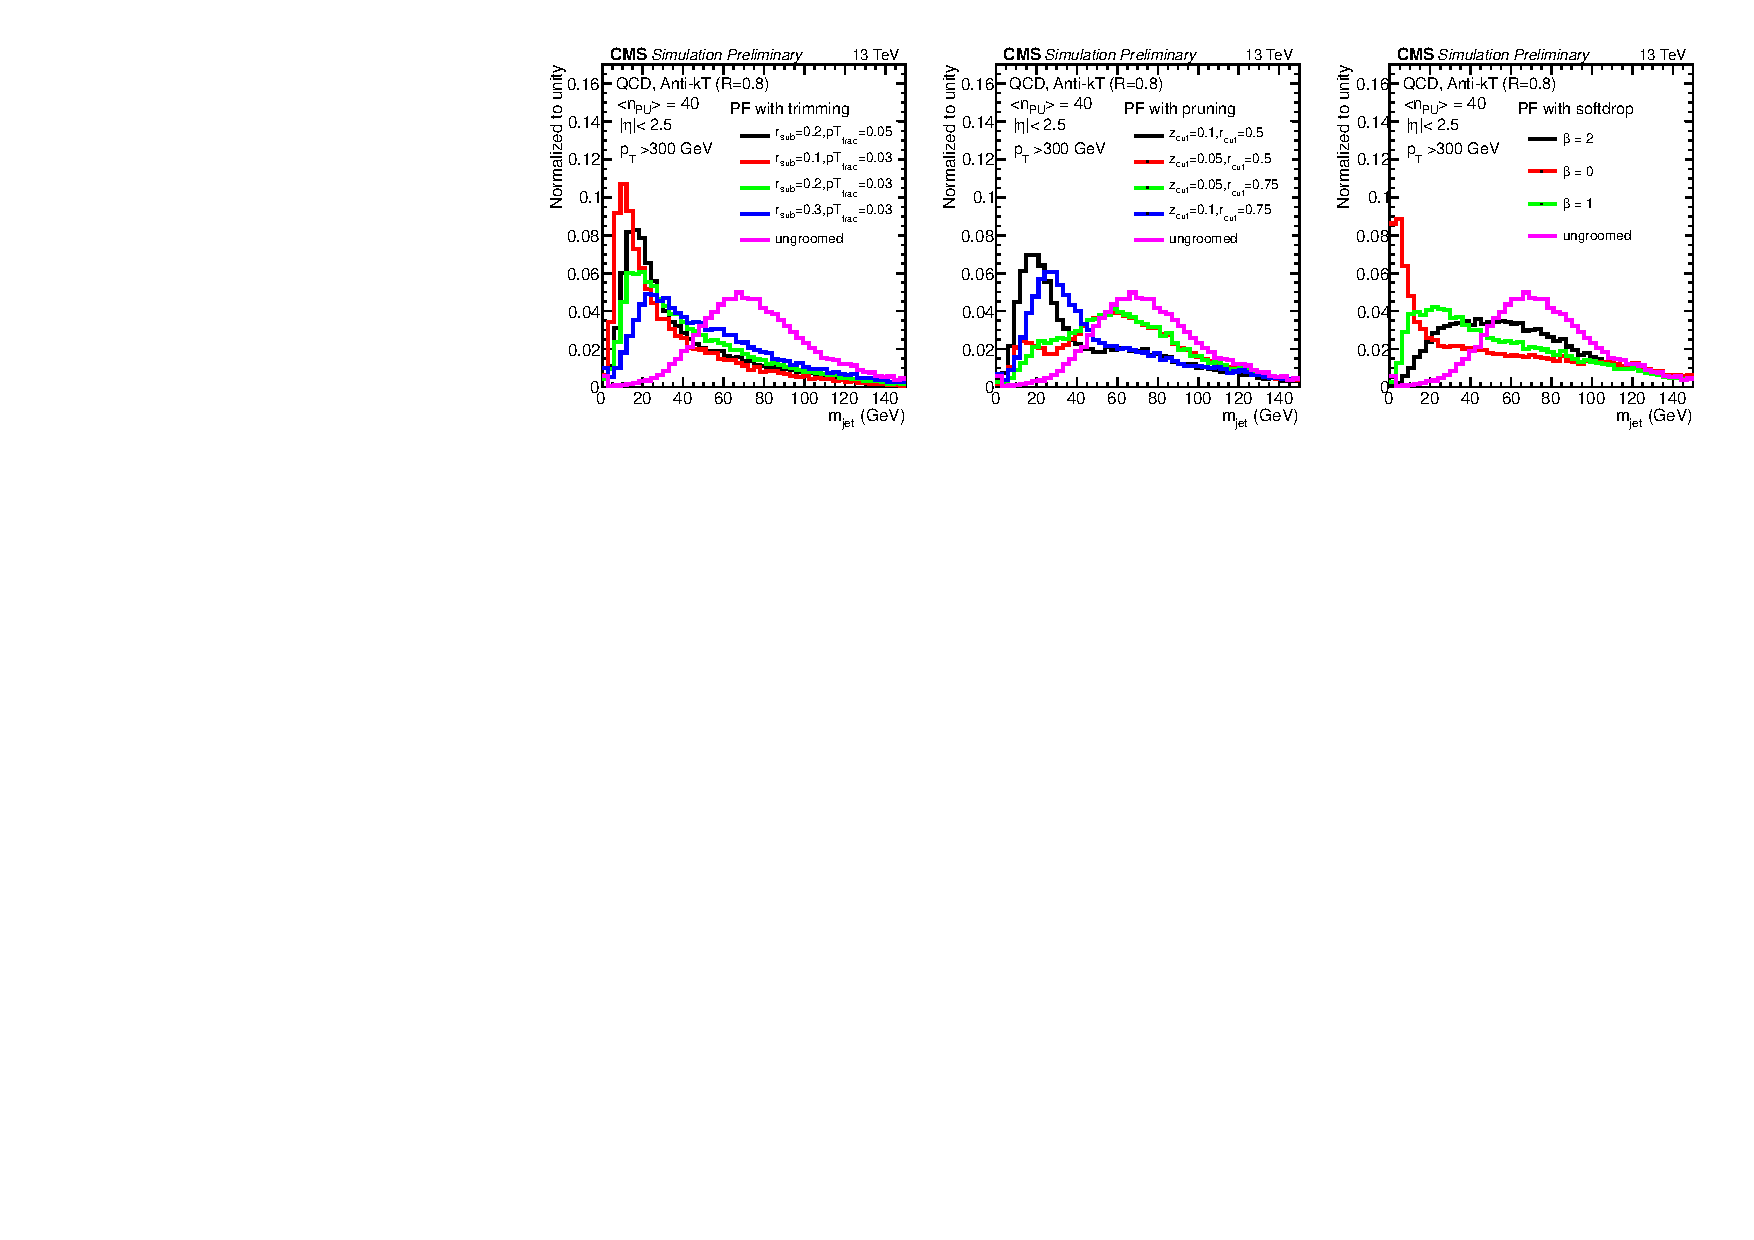
\includegraphics[width=1.00\textwidth]{/home/bibhu/Desktop/PhDThesis/PhDThesis/chapter8/1DPF_QCD.pdf}
\caption{Jet mass distributions for PF  QCD jets for different grooming parameters.}
\label{fig:jet_mass_pf_all_groomer}
\end{figure}


\begin{figure}[h]
\centering
%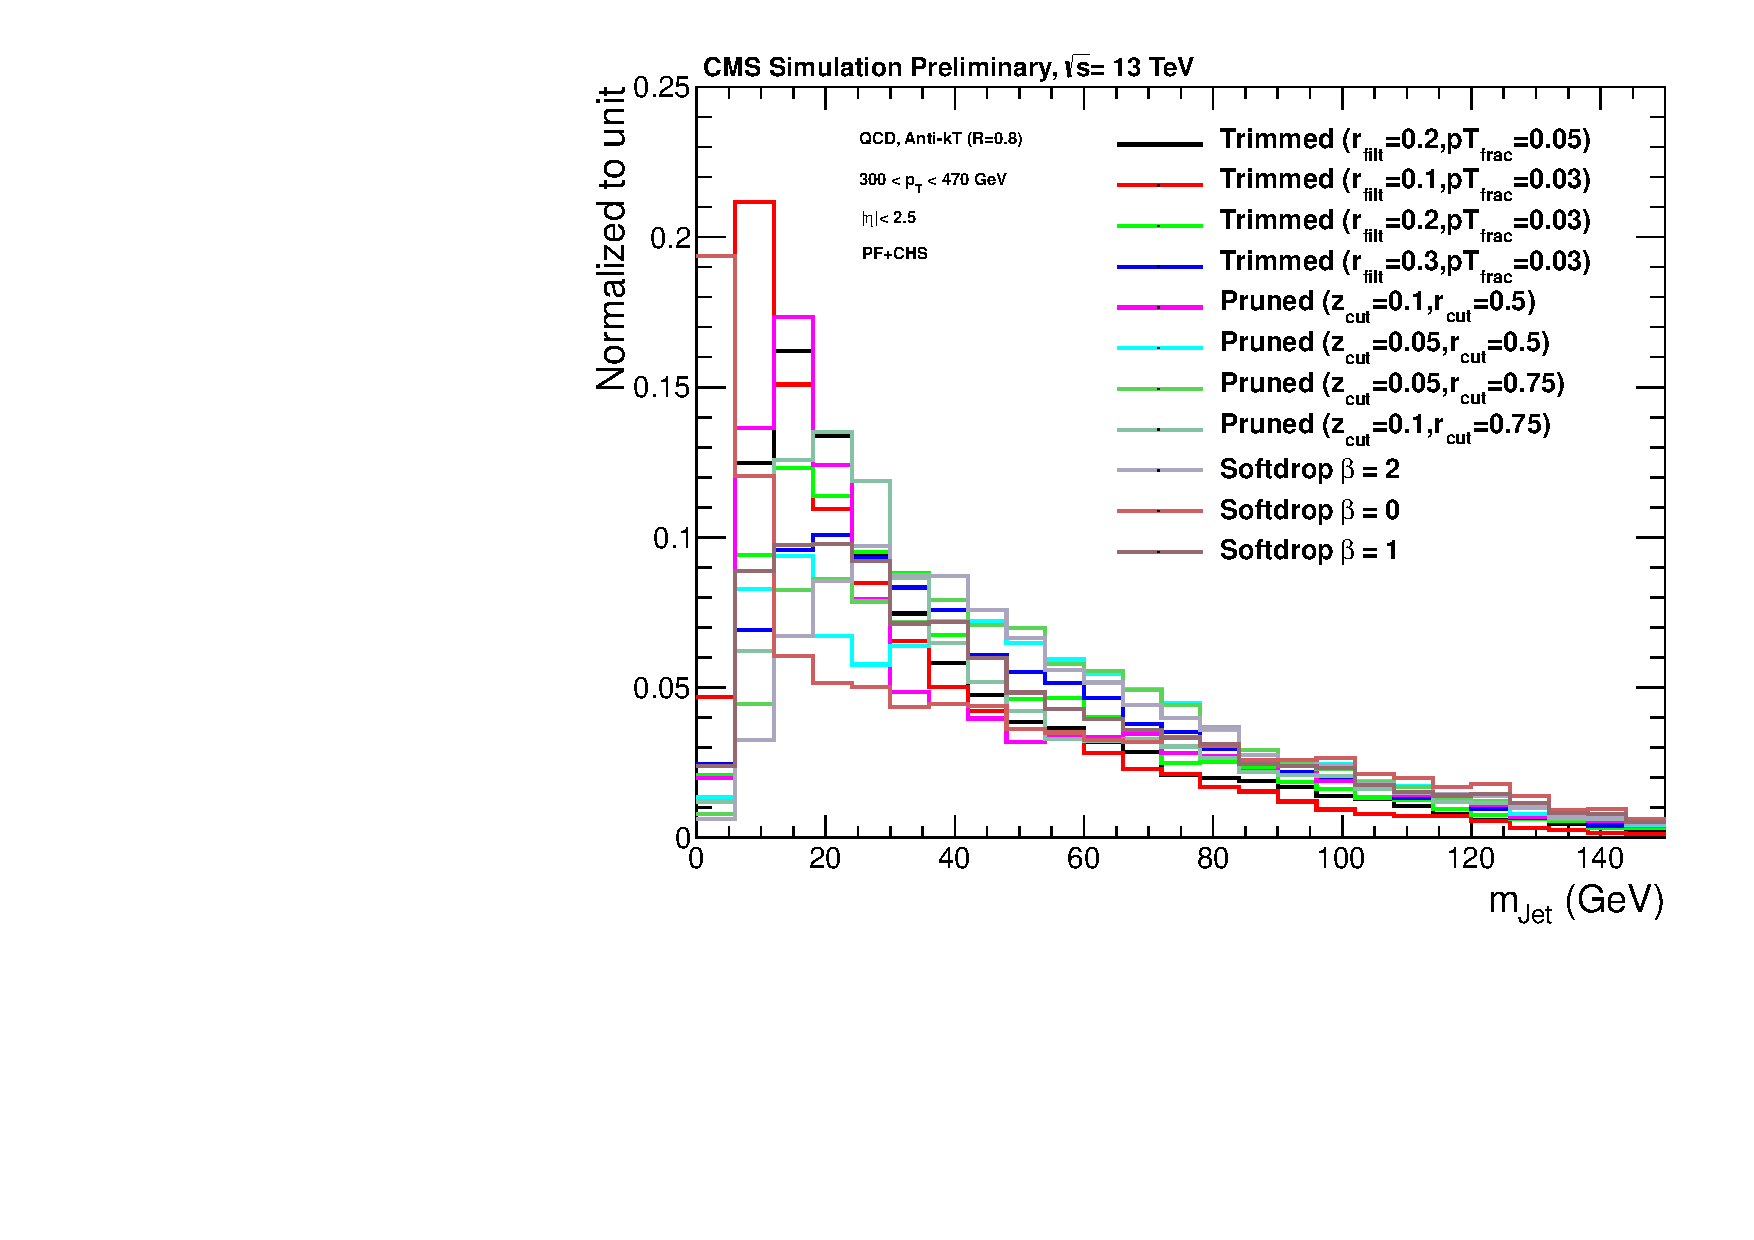
\includegraphics[width=0.60\textwidth]{Figures/puMit/Bibhu/QCD_all_groomer.pdf}
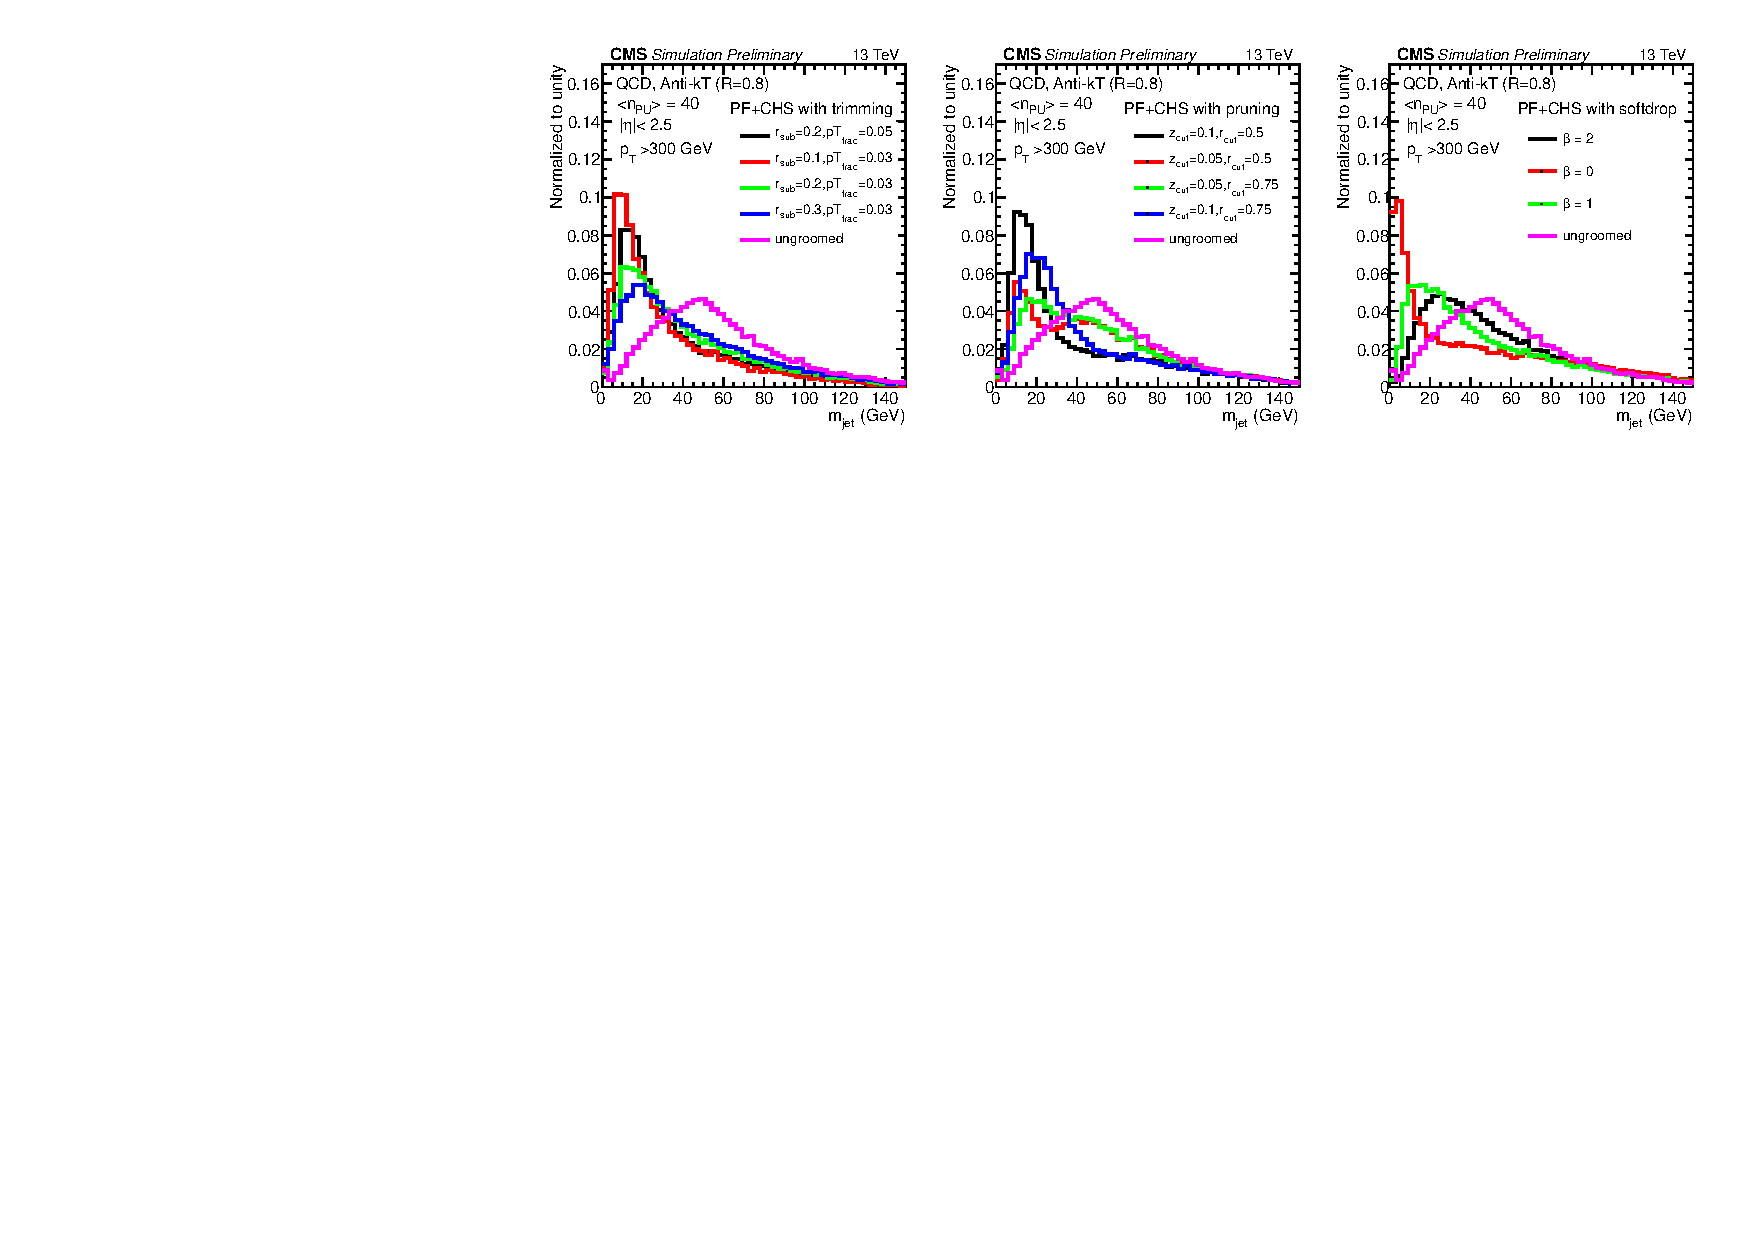
\includegraphics[width=1.00\textwidth]{/home/bibhu/Desktop/PhDThesis/PhDThesis/chapter8/1DPFCHS_QCD.pdf}
\caption{Jet mass distributions for PF+CHS  QCD jets for different grooming parameters.}
\label{fig:jet_mass_chs_all_groomer}
\end{figure}



\begin{figure}[h]
\centering
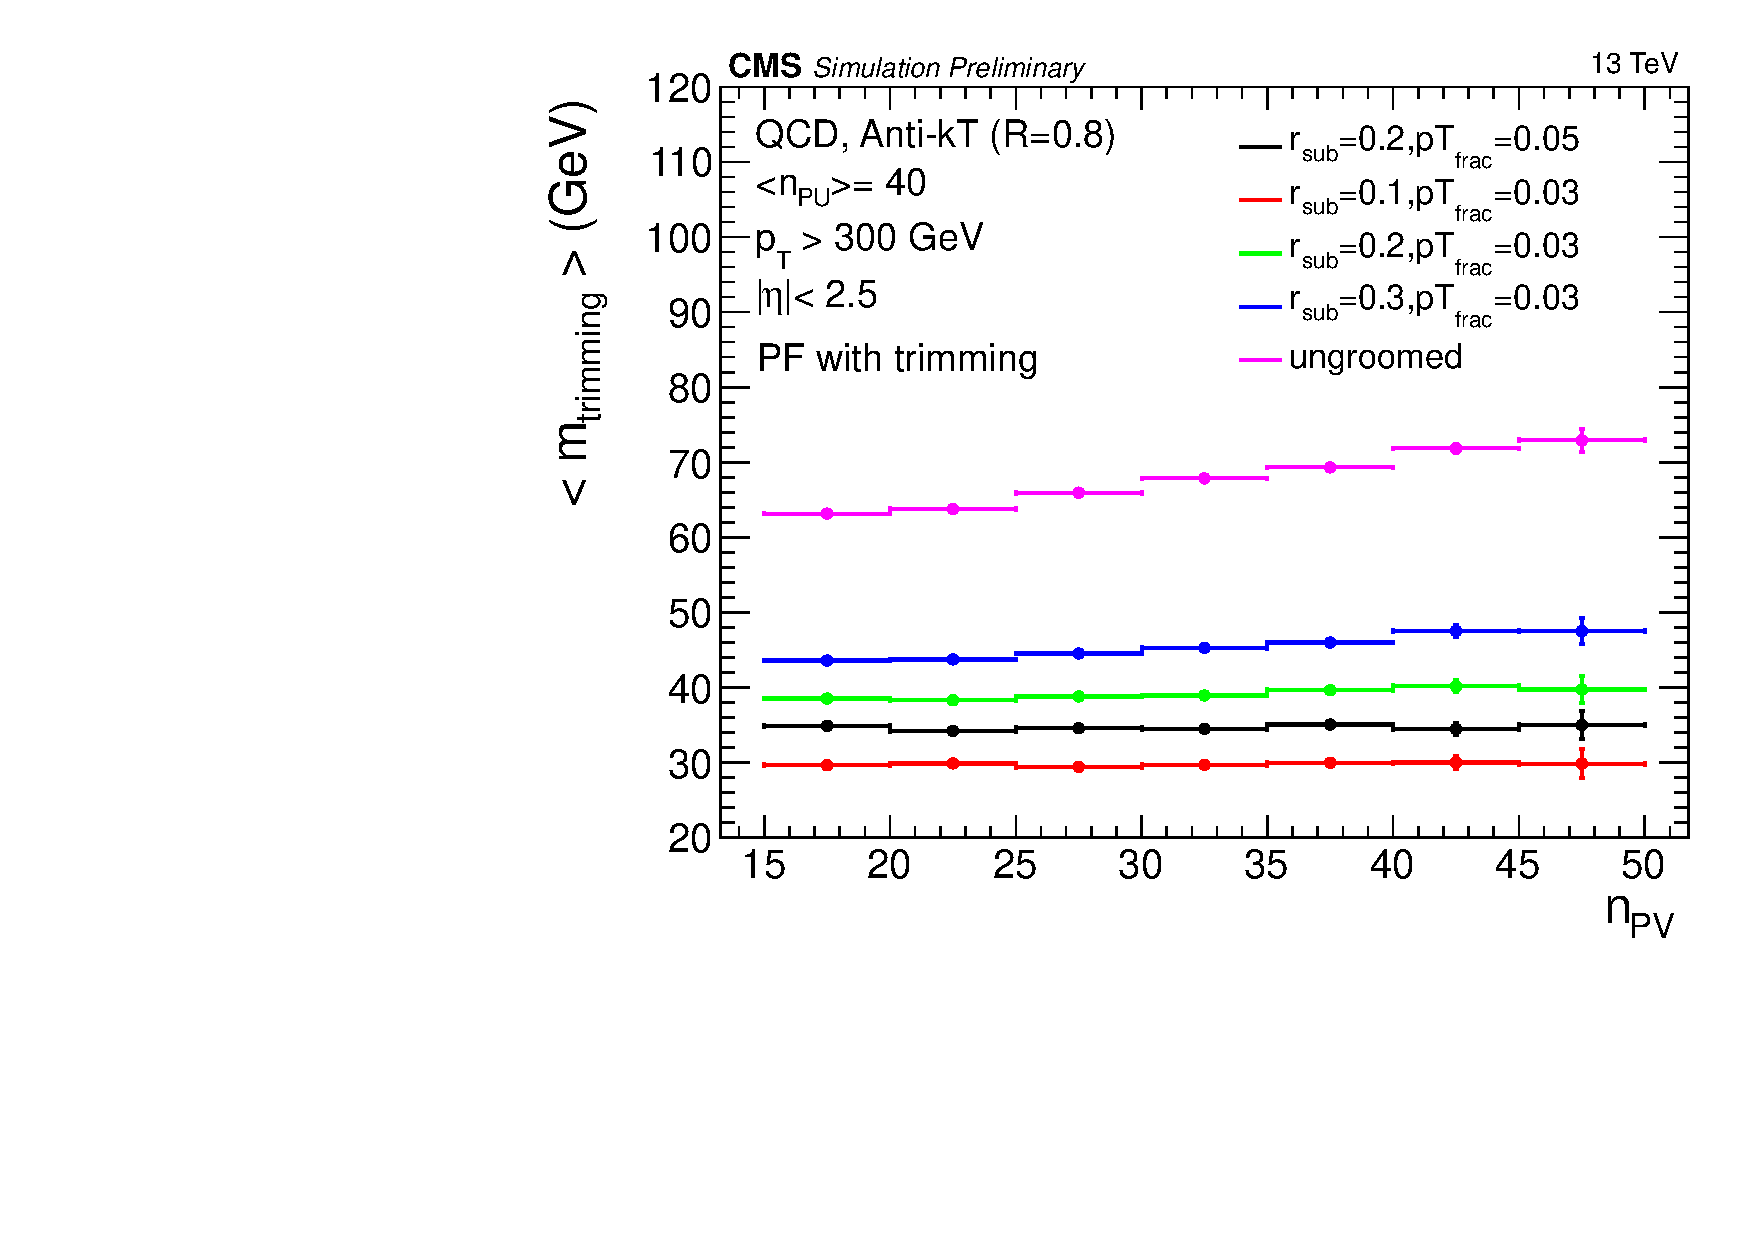
\includegraphics[width=0.47\textwidth]{/home/bibhu/Desktop/PhDThesis/PhDThesis/chapter8/AvJetmass_Vs_nPV_PF_trim.pdf}
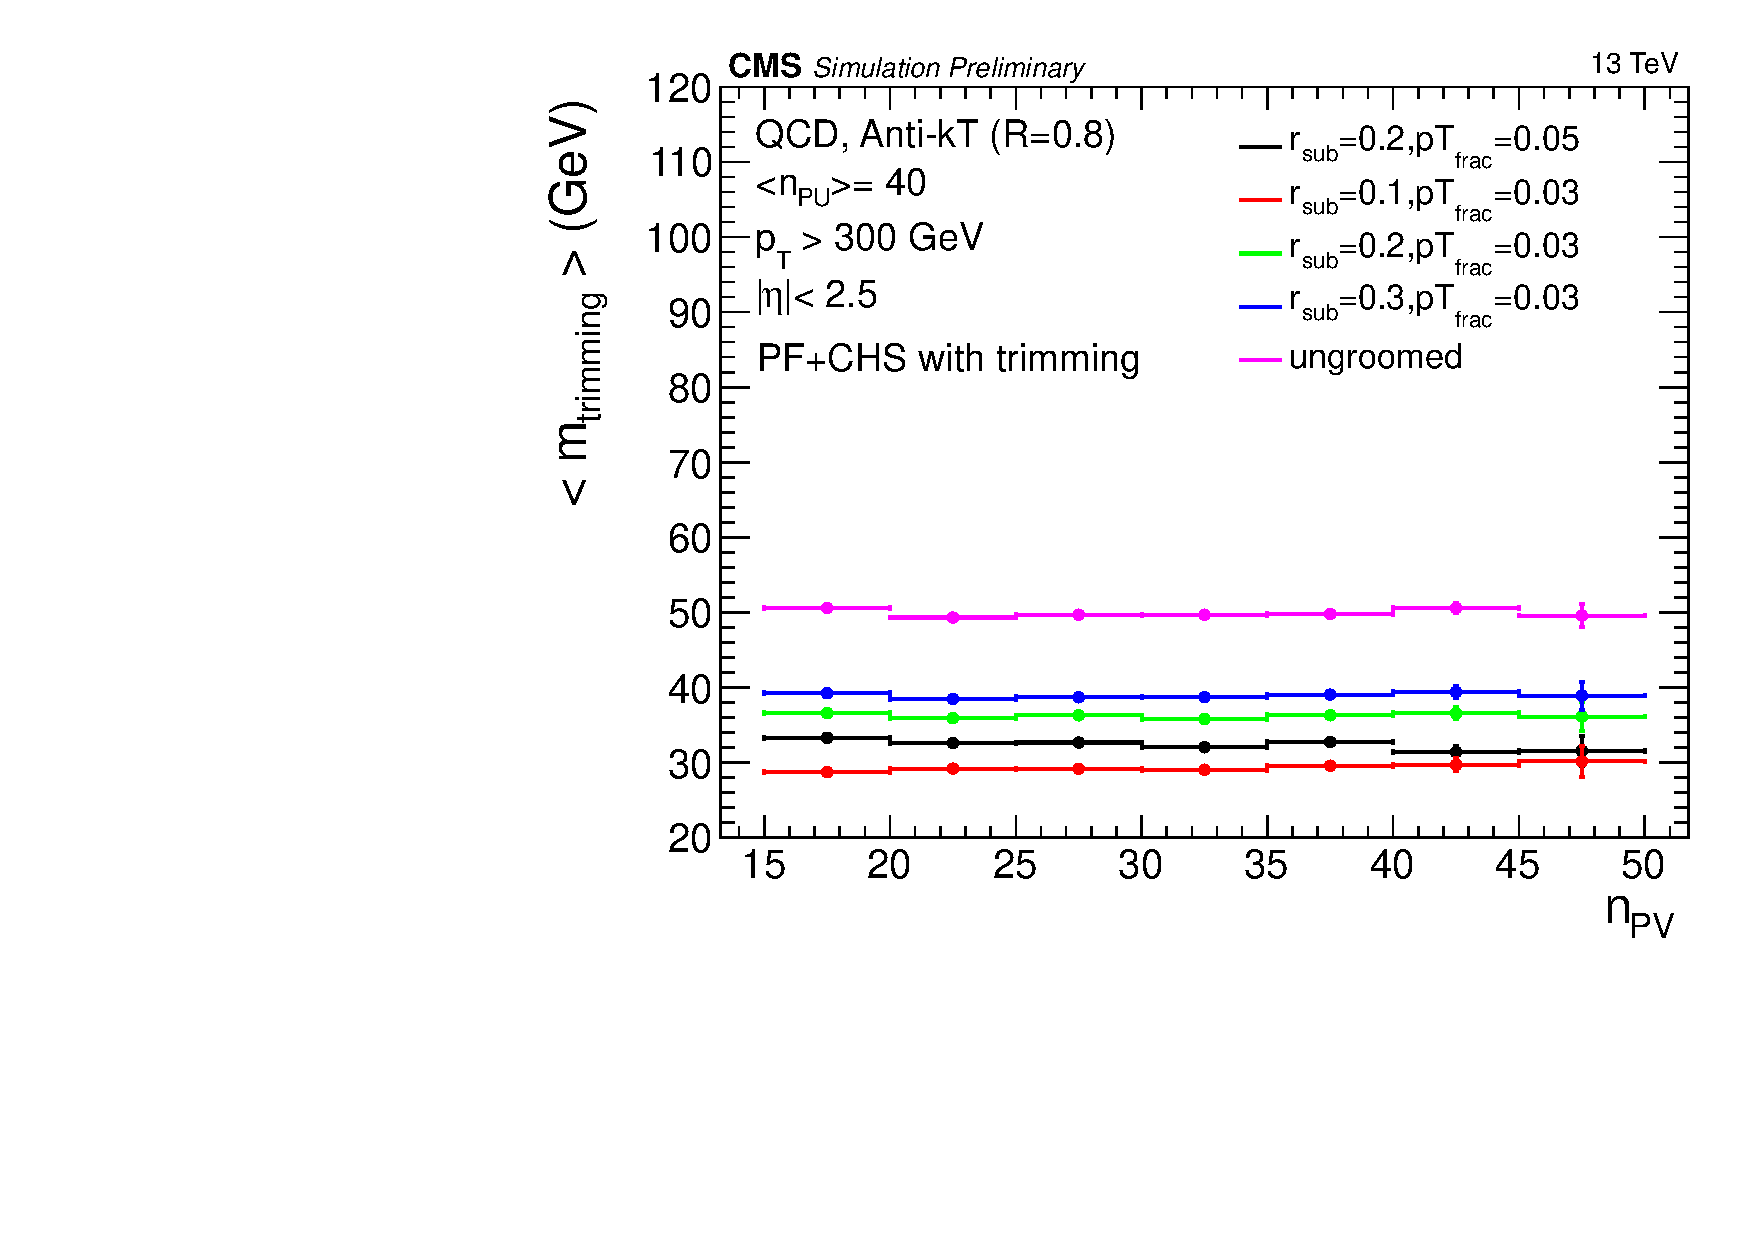
\includegraphics[width=0.47\textwidth]{/home/bibhu/Desktop/PhDThesis/PhDThesis/chapter8/AvJetmass_Vs_nPV_PFCHS_trim.pdf}\\
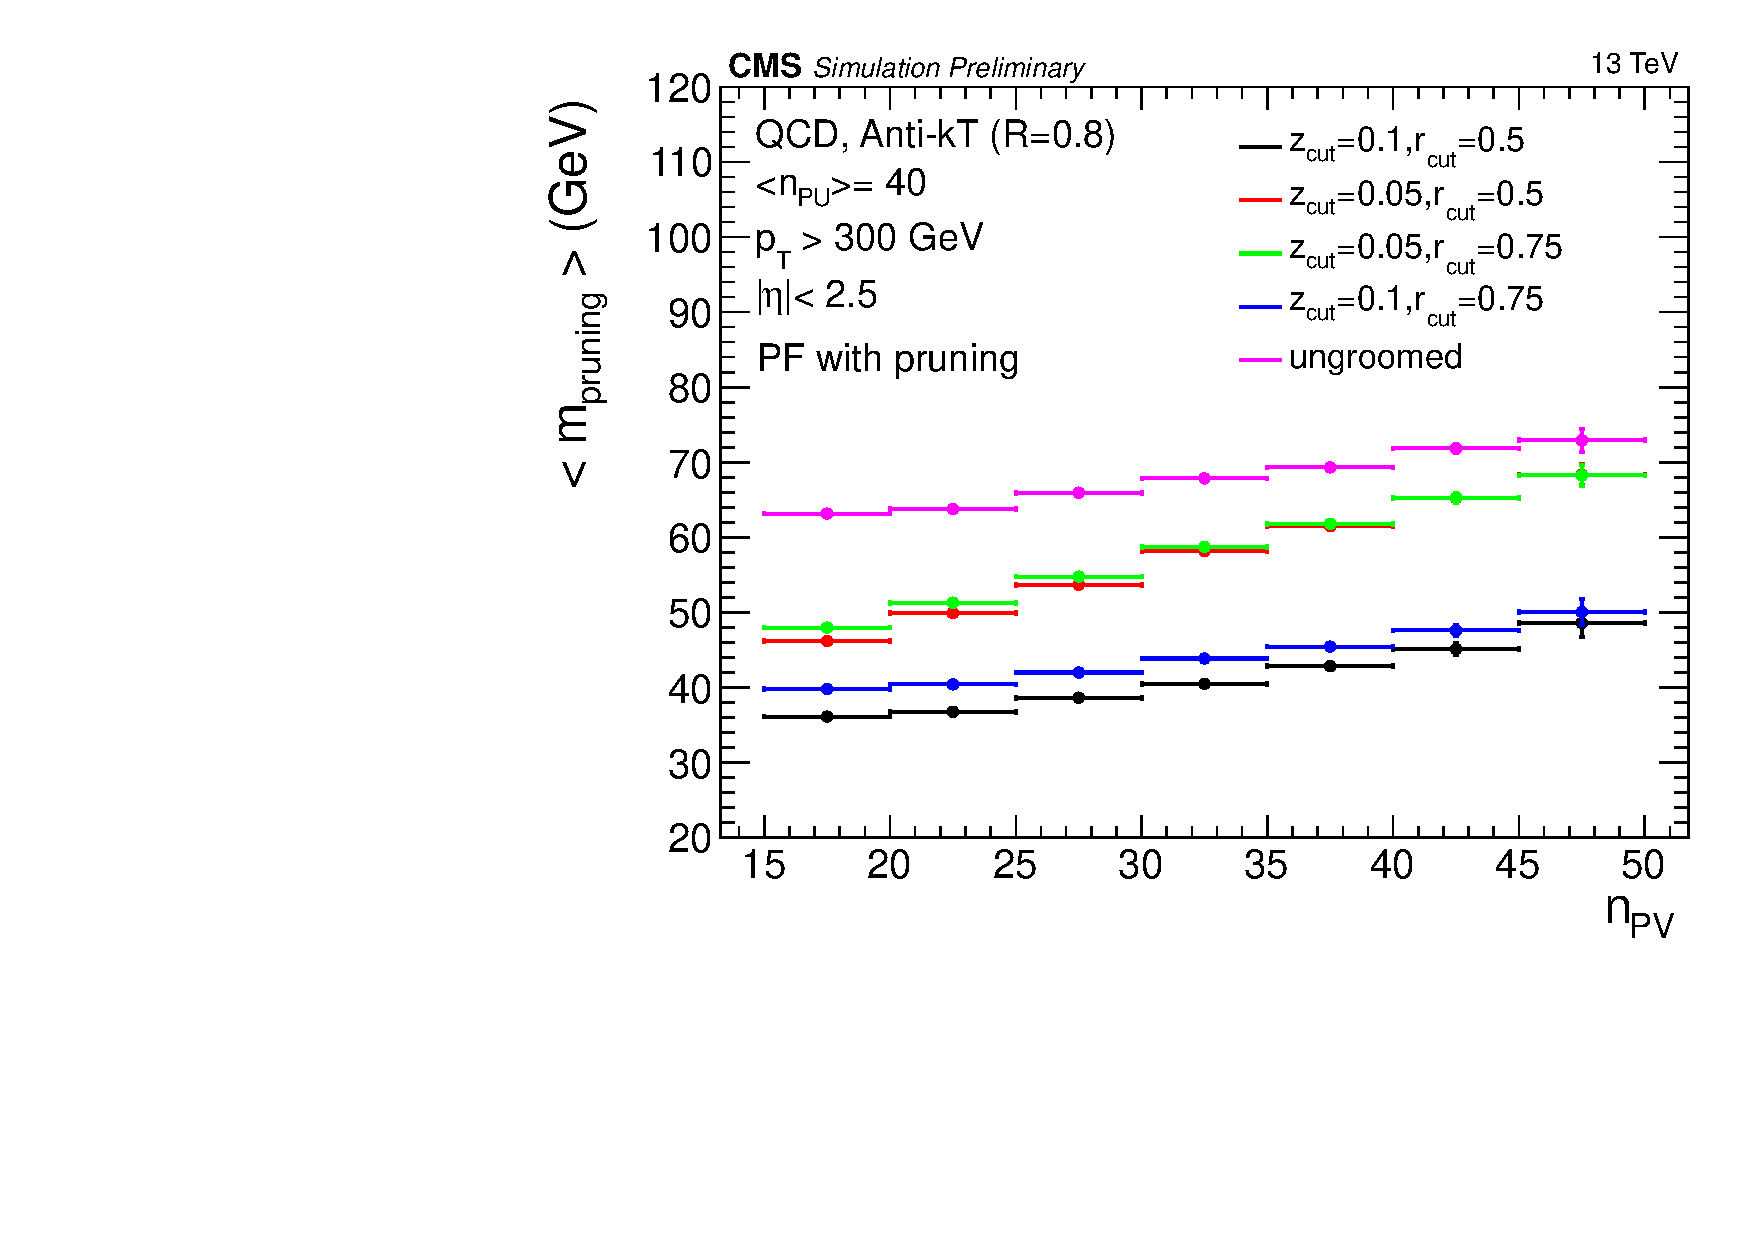
\includegraphics[width=0.47\textwidth]{/home/bibhu/Desktop/PhDThesis/PhDThesis/chapter8/AvJetmass_Vs_npv_PF_prun.pdf}
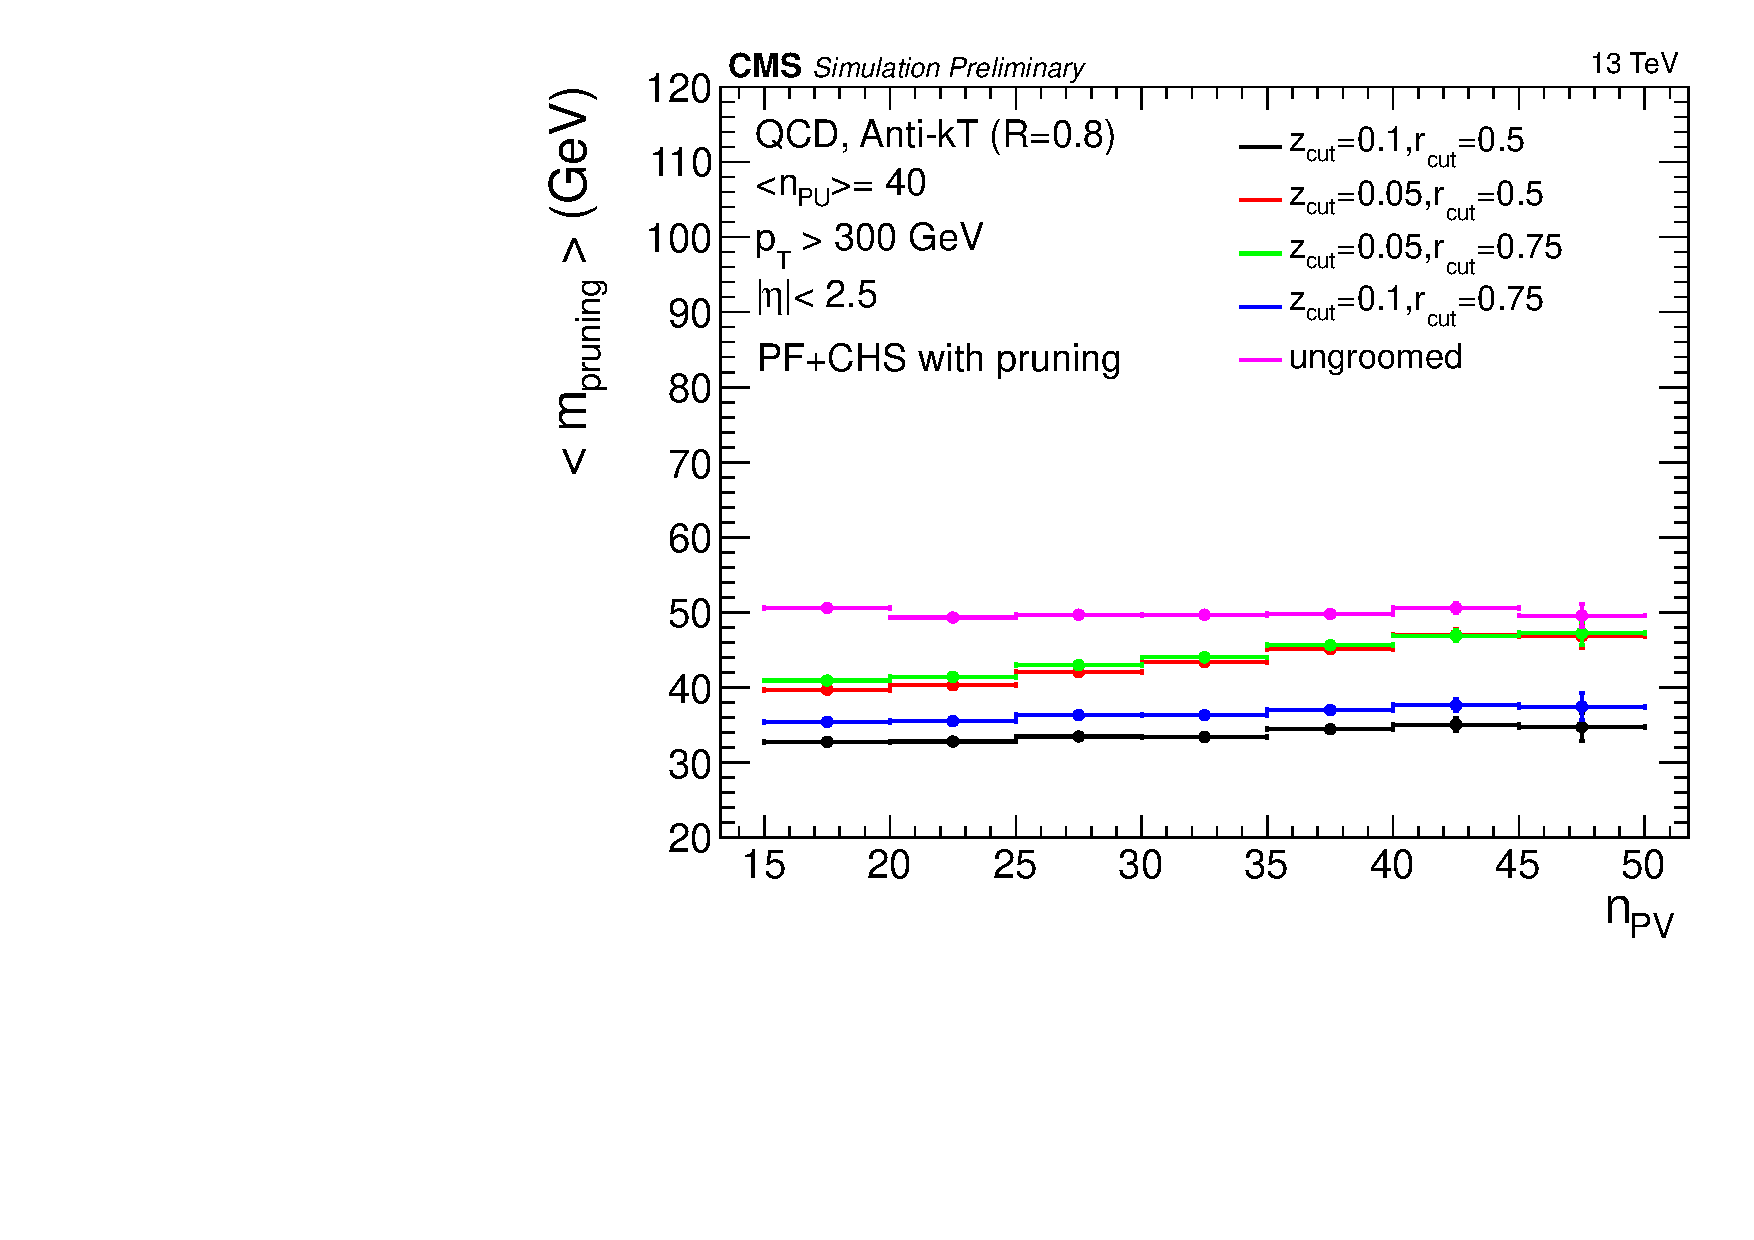
\includegraphics[width=0.47\textwidth]{/home/bibhu/Desktop/PhDThesis/PhDThesis/chapter8/AvJetmass_Vs_nPV_PFCHS_prun.pdf}\\
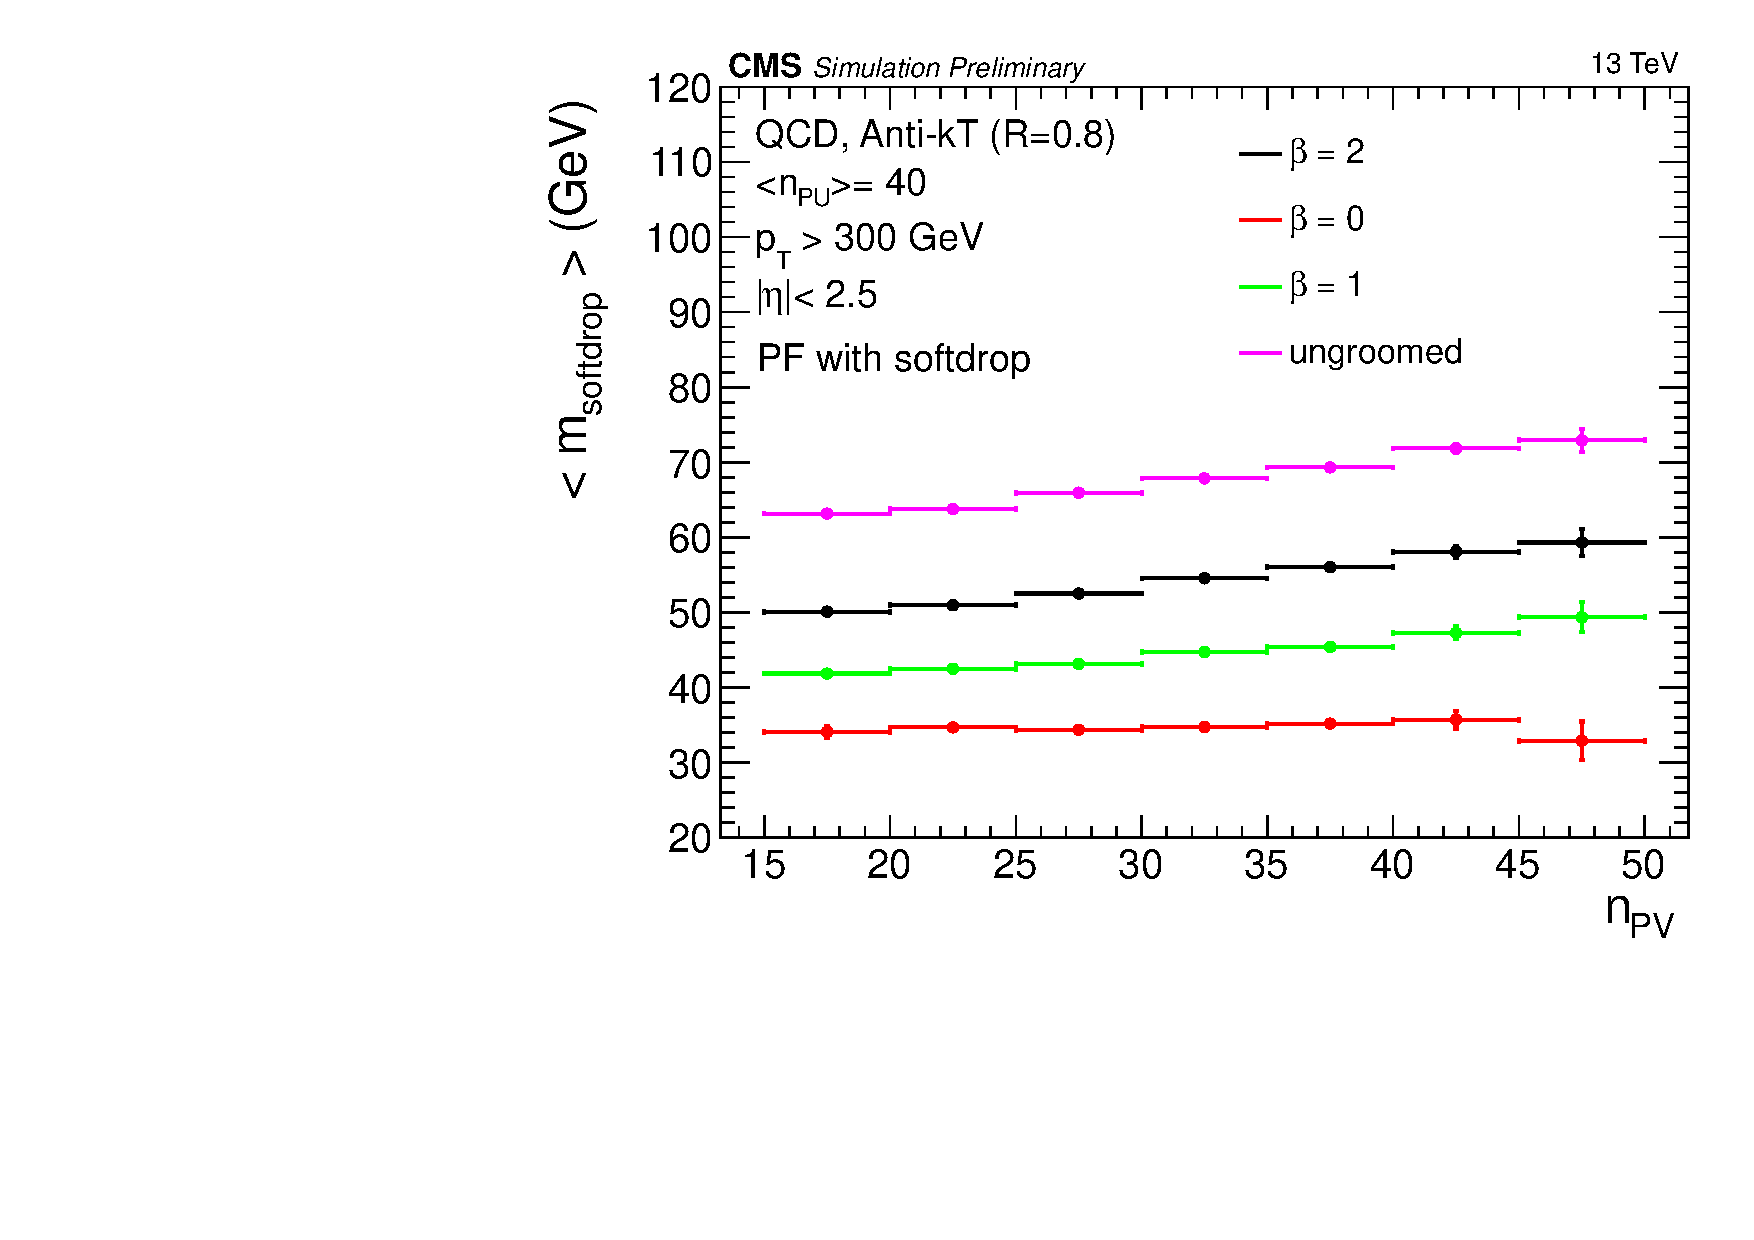
\includegraphics[width=0.47\textwidth]{/home/bibhu/Desktop/PhDThesis/PhDThesis/chapter8/AvJetmass_Vs_nPV_PF_SD.pdf}
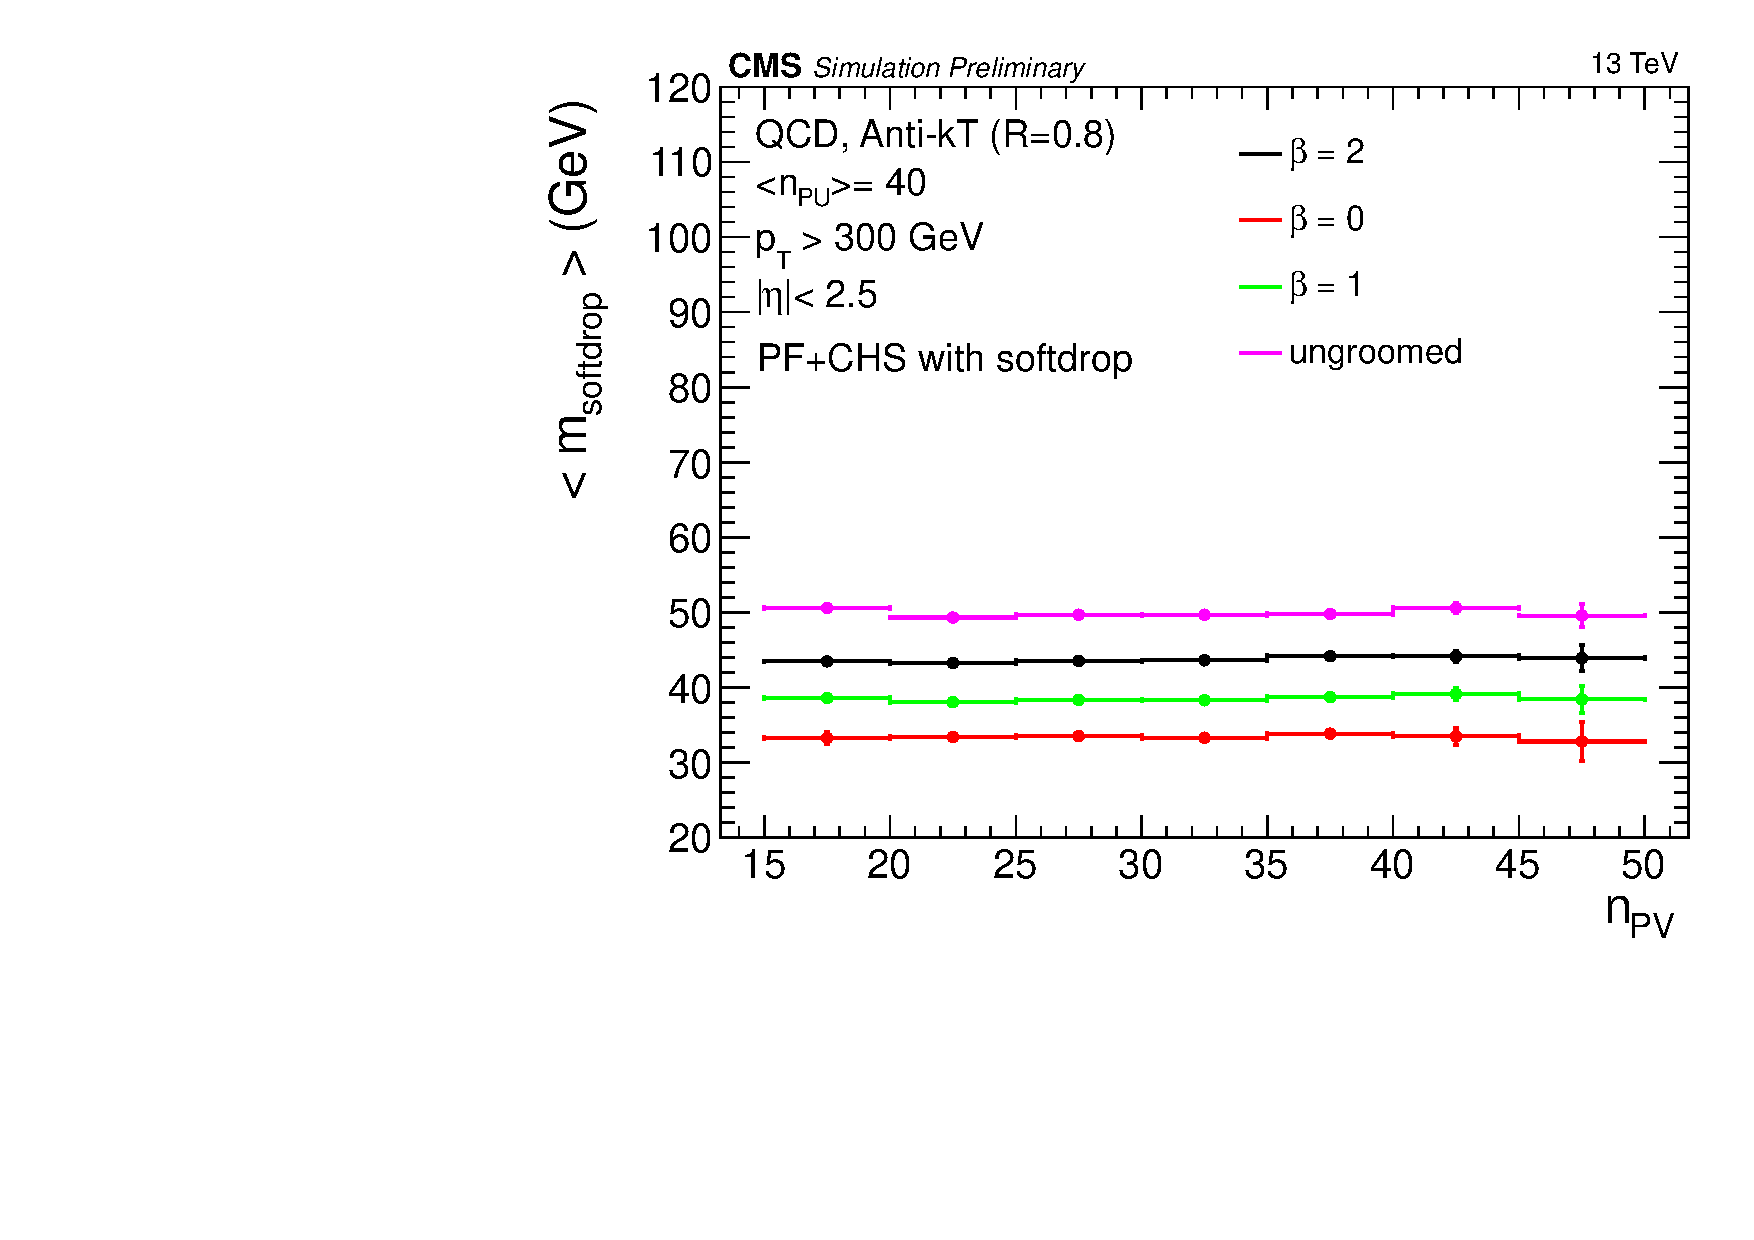
\includegraphics[width=0.47\textwidth]{/home/bibhu/Desktop/PhDThesis/PhDThesis/chapter8/AvJetmass_Vs_nPV_PFCHS_SD.pdf}\\
\caption{Pileup dependence of the average jet mass for PF jets (left) and PF+CHS jets (right) for various grooming algorithms and parameters.}
\label{fig:grooming_PFvCHS}
\end{figure}


We also compare the resolution of jets after the application of various grooming algorithms by plotting the RMS values from the jet response templates. Fig.~\ref{fig:summary_all_groomer_QCD} shows that trimming has better mass resolution followed by soft-drop and pruning.



\begin{figure}[h]
\centering
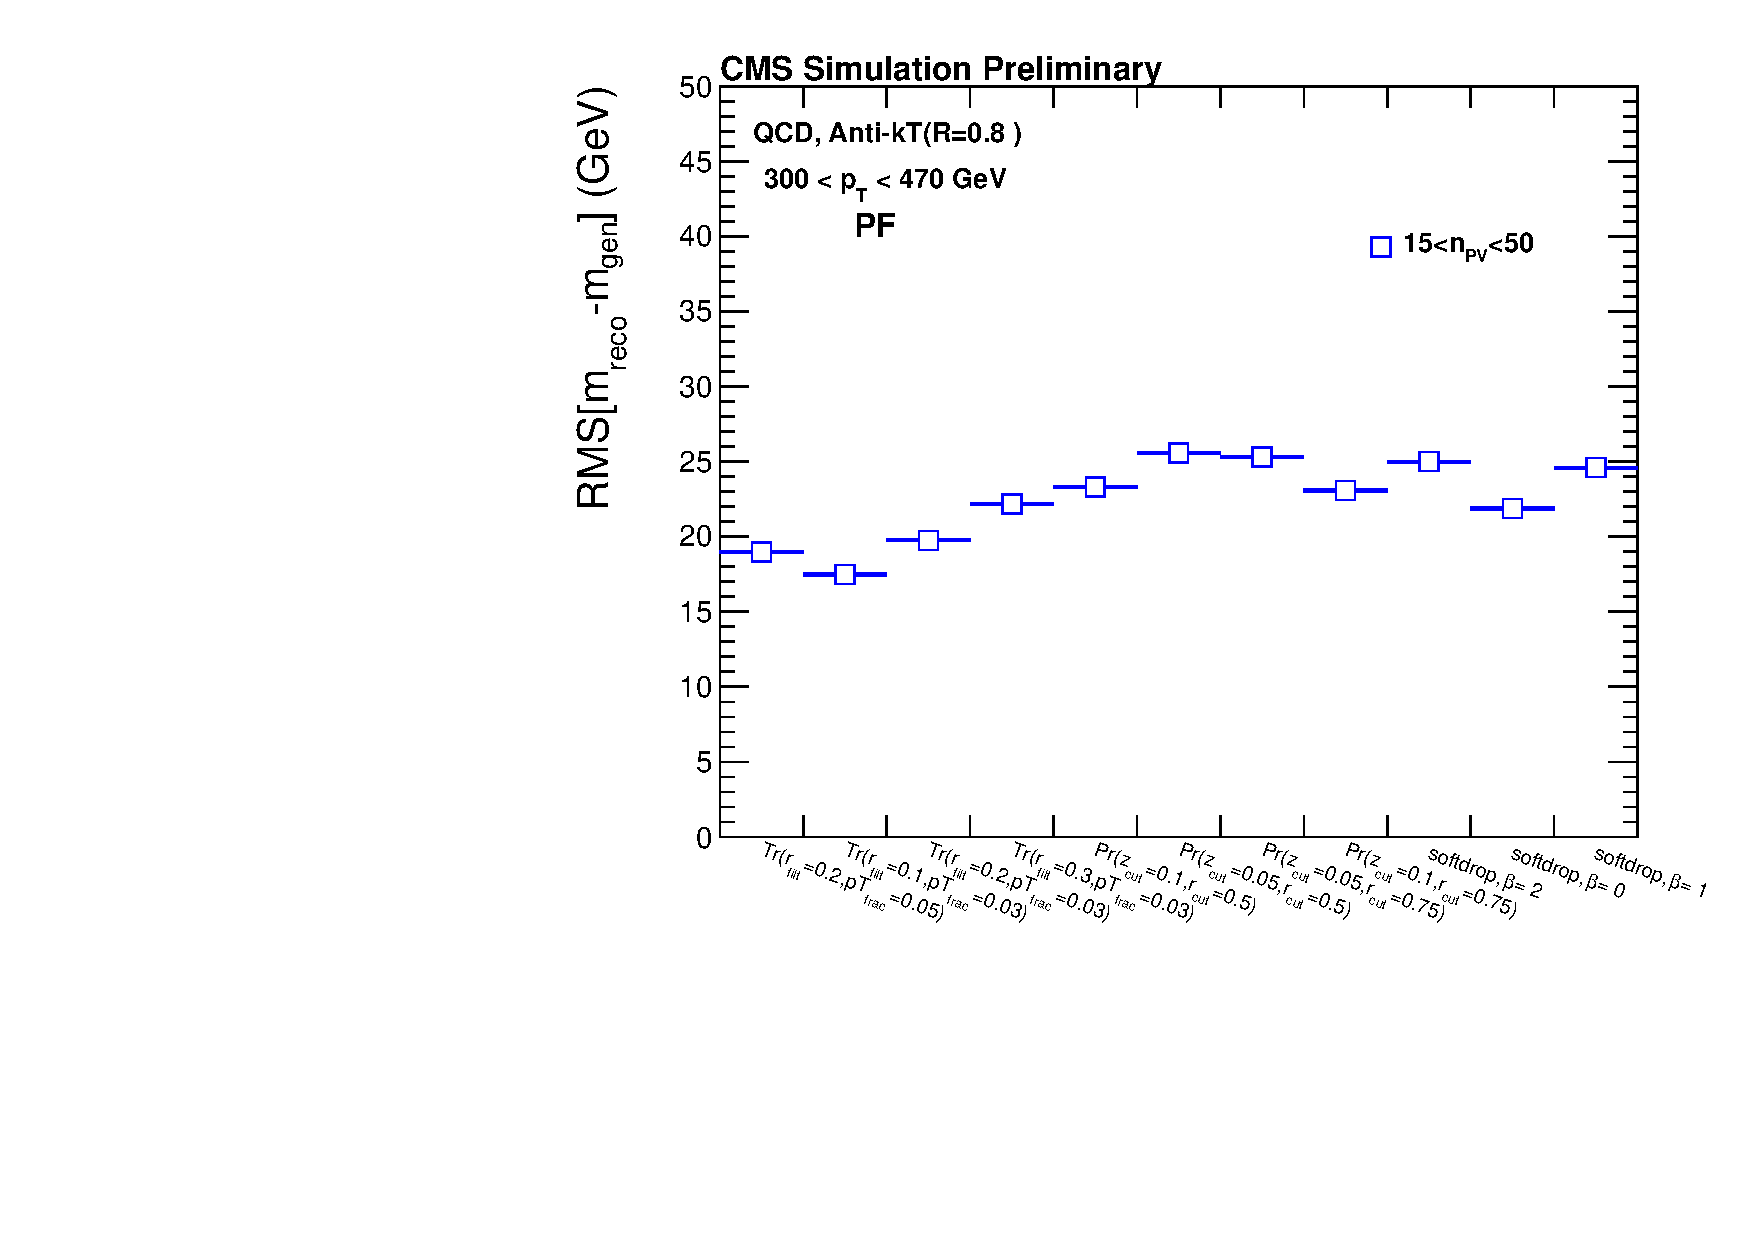
\includegraphics[width=0.47\textwidth]{/home/bibhu/Desktop/PhDThesis/PhDThesis/chapter8/SummaryPFallNPV.pdf}
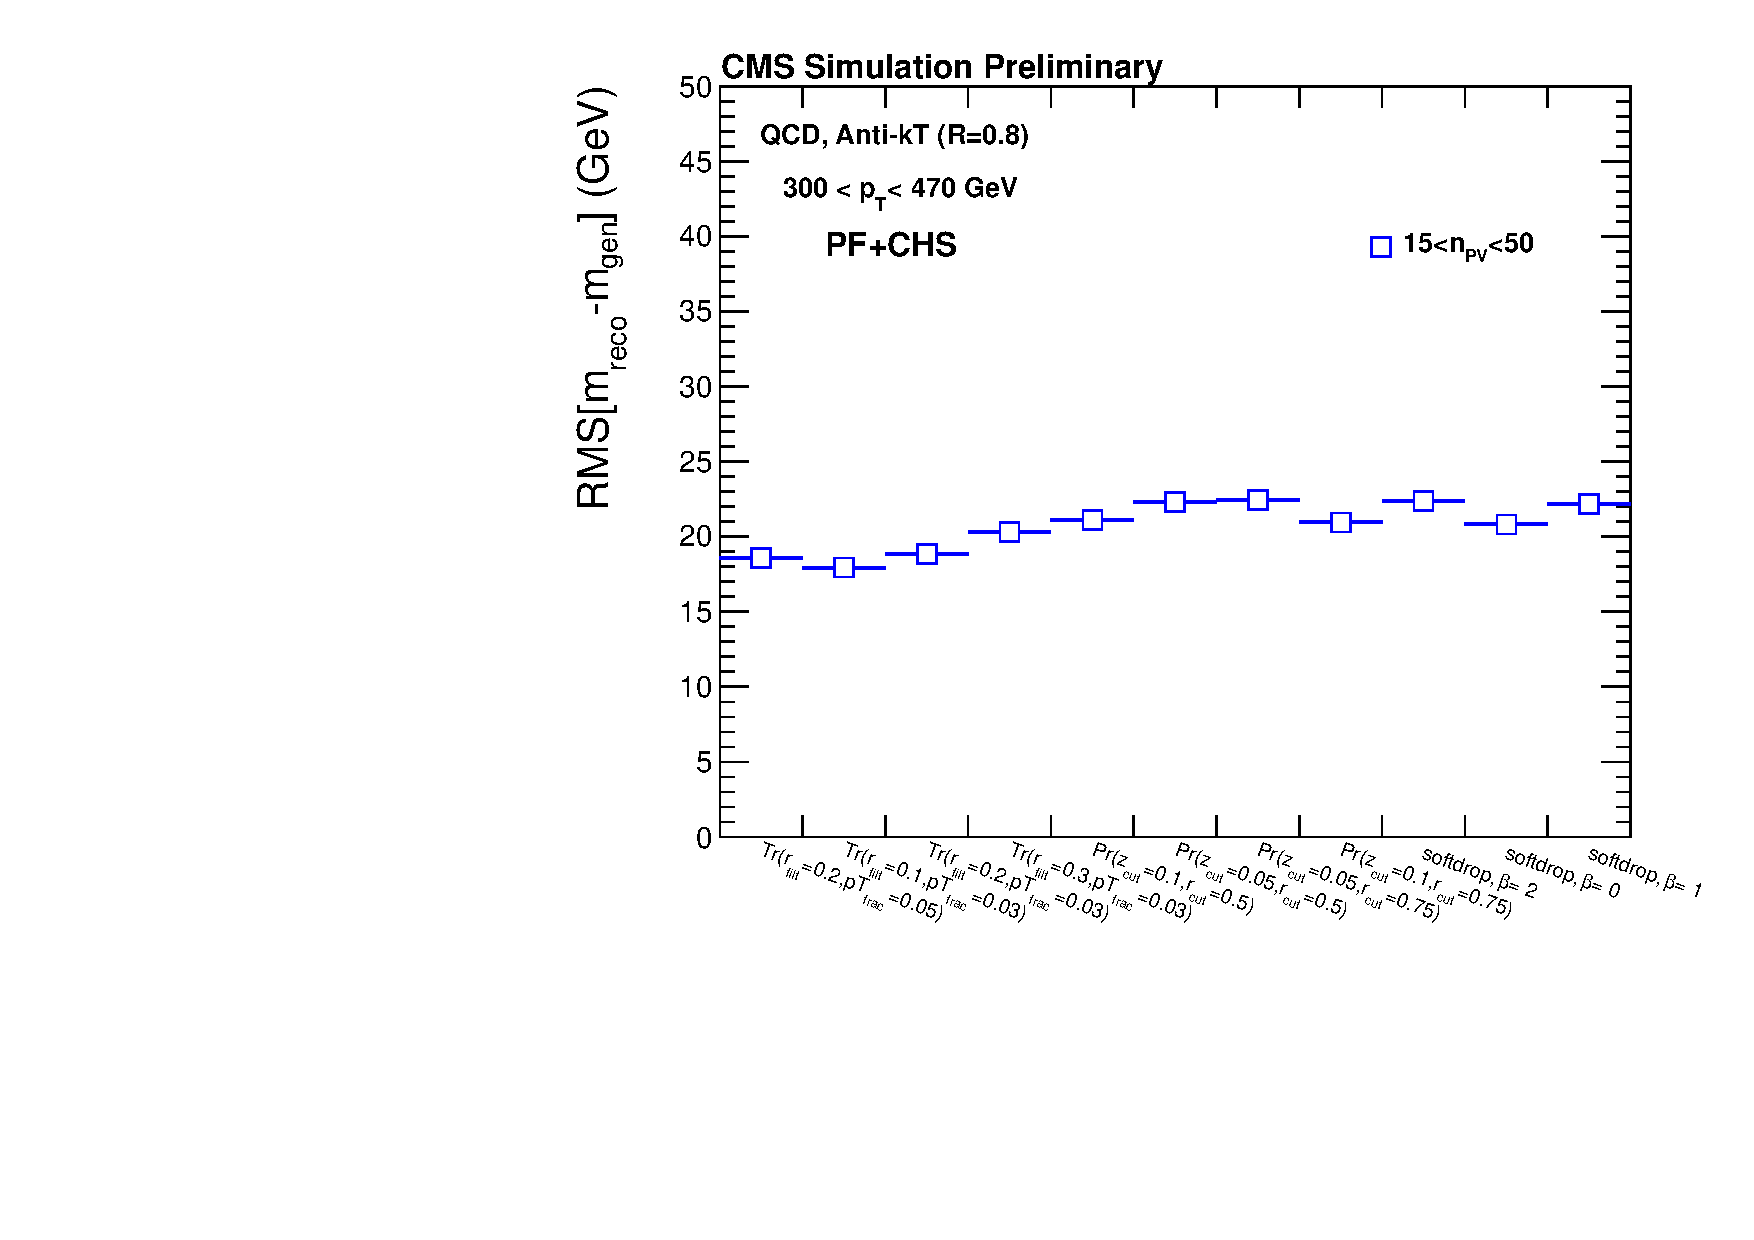
\includegraphics[width=0.47\textwidth]{/home/bibhu/Desktop/PhDThesis/PhDThesis/chapter8/SummaryPFCHSallNPV.pdf}\\
\caption{Comparison of jet mass resolution for PF and PF+CHS  with different grooming algorithms and parameters.}
\label{fig:summary_all_groomer_QCD}
\end{figure}
















